\documentclass{article}
\usepackage{float}
\usepackage{graphicx}
\usepackage{amsmath}
\usepackage{blindtext}
\usepackage[none]{hyphenat}
\usepackage{chngcntr}
\usepackage[section]{placeins}
\usepackage{subcaption}
\usepackage{anysize}
\usepackage{enumerate} 
\usepackage{titlesec}
\titleclass{\subsubsubsection}{straight}[\subsection]
\newcounter{subsubsubsection}[subsubsection]
\renewcommand\thesubsubsubsection{\thesubsubsection.\arabic{subsubsubsection}}
\titleformat{\subsubsubsection}
  {\normalfont\normalsize\bfseries}{\thesubsubsubsection}{1em}{}
\titlespacing*{\subsubsubsection}
{0pt}{3.25ex plus 1ex minus .2ex}{1.5ex plus .2ex}

\makeatletter
\renewcommand\paragraph{\@startsection{paragraph}{5}{\z@}%
  {3.25ex \@plus1ex \@minus.2ex}%
  {-1em}%
  {\normalfont\normalsize\bfseries}}
\renewcommand\subparagraph{\@startsection{subparagraph}{6}{\parindent}%
  {3.25ex \@plus1ex \@minus .2ex}%
  {-1em}%
  {\normalfont\normalsize\bfseries}}
\def\toclevel@subsubsubsection{4}
\def\toclevel@paragraph{5}
\def\toclevel@paragraph{6}
\def\l@subsubsubsection{\@dottedtocline{4}{7em}{4em}}
\def\l@paragraph{\@dottedtocline{5}{10em}{5em}}
\def\l@subparagraph{\@dottedtocline{6}{14em}{6em}}
\makeatother

\setcounter{secnumdepth}{4}
\setcounter{tocdepth}{4}


\begin{document}

\renewcommand{\figurename}{\textbf{Figure}} 
\renewcommand\thefigure{\textbf{\arabic{figure}}} 
\counterwithin{figure}{section}




\section{Infering radius}

If we look at the equation \ref{velocity_equation} we can see that in the case we are dealing with there are three main unknown parameters if we consider that we are acquiring the velocity from the data space supplied by the experimental part. These parameters are the radius, the density and the drag coefficient. Note also that ,additionally to the velocity, we are getting information of the droplet radius in each sample.
\par \noindent
The main idea of this first scenario  is setting the drag coefficient as a constant value. With this approach the  model is more restrictive in the sense that we are allowing  only uncertainties in two parameters: the radius and the density.
\par \noindent

\begin{subsubsubsection}{Drag Coefficient approximation}

Taking this into account, the inverse problem resolution will be based on the unknown  two parameters. At this point is important to approximate the fixed variable ( drag coefficient) to the most certain value. Usually the drag coefficient is obtained balancing the forces actuation over a body But in this case, we don't have any information regarding to the forces, so we need to approximate the drag coefficient somehow. One option is using  tabulated values that comes from experiments but the problem is that  the majority of this experiments are based on air or in solid bodies. For that reason  in this specific problem, we are going to consider  a polynomial  expression from \ref{morrison2013data} which expresses the drag coefficient in function of the Reynolds Number: 

\begin{equation} \label{eq:drag_coefficient}
C_d=\frac{24}{Re}+\frac{2.6\left(\frac{Re}{5.0}\right)}{1+\left(\frac{Re}{5.0}\right)^{1.52}}+\frac{0.411\left(\frac{Re}{2.63\dot 10^5}\right)^{-7.94}}{1+\left(\frac{Re}{2.63\dot 10^5}\right)^{-8.00}}\\
\end{equation}

Where the Reynolds Number is calculated in function of the droplet radius $r_d$ , the water density $\rho$ and the kinematic viscosity $\mu$:
\begin{equation} \label{eq:Reynolds}
Re=\frac{\rho r_d U_d}{\mu}\\
\end{equation}

Thus, using the experimental data, the drag coefficient has been calculated for each sample and taking the average of those values
 we get an approximation for the drag coefficient which is approximately $0.77$ it seems quite large for the typical value of a sphere in a fluid ( around $0.5$) but will be our first approximation. Knowing the exact vale for  the droplet density we can approximate this value using the physical model [\ref{eq:velocity_function}]. In this case we get a value over $1.25$. As we have two dissimilar values we will solve the inverse problem for those values and two more in order to study their influence in the posterior distribution.
 
\end{subsubsubsection} 
 \par \noindent
 
 
\subsubsubsection{Inferring Radius Results}

Once we know the unknown and the fixed parameters, we can study the inverse problem and solve it using the application. As it has been described before, for the resolution, QUESO needs two inputs files.The \textit{$queso.in$} describes basically the QUESO resolution options and the \textit{$model_input.in$} which describes the main characteristics of the scenario:
\begin{enumerate}
\item For establishing the prior, the application needs information \textit{a priori} concerning the parameters which consists in  a minimum and a maximum value for the parameters  domain. Remark that the variables will be studied in their normalized value. Thus if we want the exact value we must multiply by the nominal value.
\item In this scenario, we will give the specific value to the drag coefficient.
\item The other variables of the physical model are the water density and the gravity which are  constant values for all  scenarios.
\end{enumerate}
After setting the input file, we can solve the inverse problem and plot the posterior information using MATLAB. The idea behind the different scenarios  is to study the influence of the parameters in the posterior distribution of the density and thus validate the application. The results are validated  considering that we already know the value of the droplet density ( The value of the  castor oil density is $961 kg/m^3$) and then a good approximation would be the one which is centered around this value.





\begin{figure}[H]
\captionsetup[subfigure]{justification=centering}
\begin{center}
  \begin{subfigure}{0.4\textwidth}
    \centering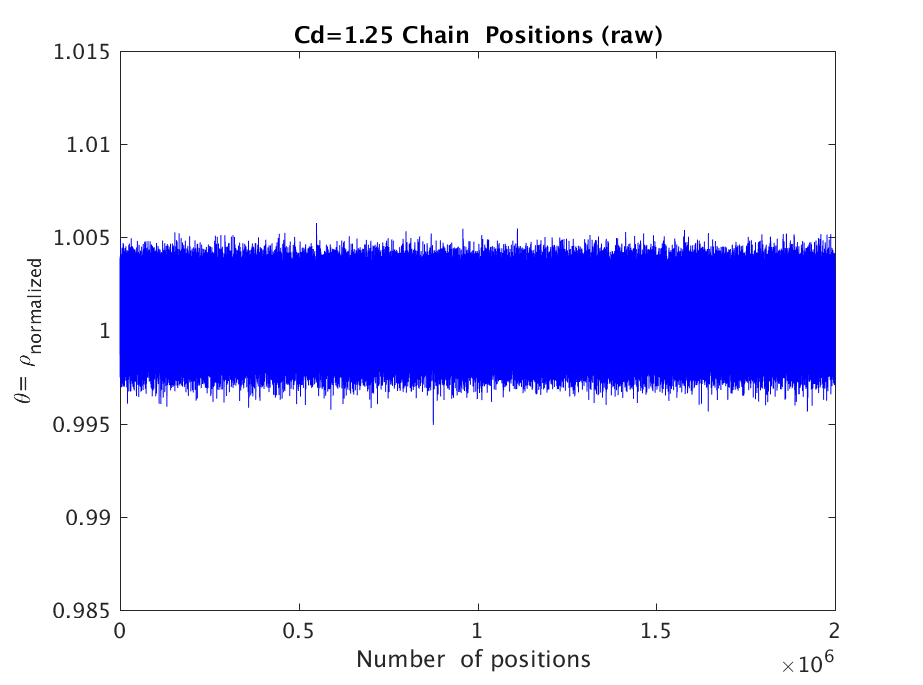
\includegraphics[width=1.1\textwidth,keepaspectratio]{images/inverse_problem/infer_radius/drag_125/range_short/density_samples_chain.png}
    \caption{\centering Raw Chain}
  \end{subfigure}
 %%\hspace{1.5cm}%
 \begin{subfigure}{0.4\textwidth}
    \centering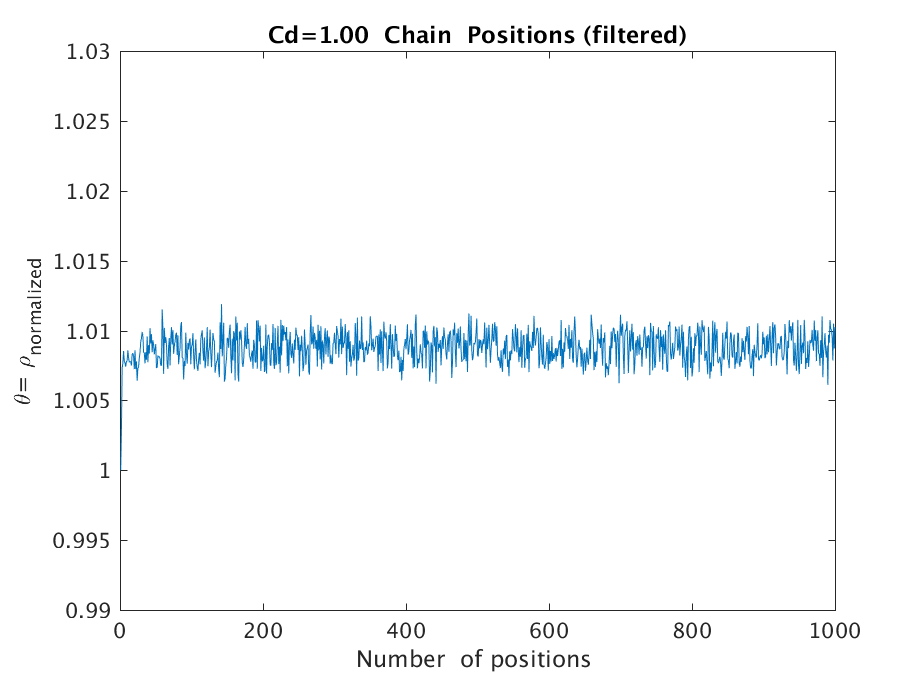
\includegraphics[width=1.1\textwidth,keepaspectratio]{images/inverse_problem/infer_radius/drag_01/density_samples_filtered.png}
    \caption{\centering Filtered Chain}
  \end{subfigure}


\caption{Markov Chain}
\label{fig:chain} 
 \end{center}
\end{figure}


Previous to show the main results, we need to make give some points from the data we get from the output files. Basically in the output files we get the samples of the Markov Chain and using this data we get the information related to the parameters such as the histograms, the density distribution,...Looking at this chains, one can appreciate if the samples fits with the interval set for the prior distribution.
In the figure (\ref{fig:chain}) we can see the shape of either the raw chain and the filtered. Concerning to the second one it  will be shown later that aims to have the same information than the whole chain.



\begin{figure}[H]
\captionsetup[subfigure]{justification=centering}
\begin{center}
  \begin{subfigure}{0.4\textwidth}
    \centering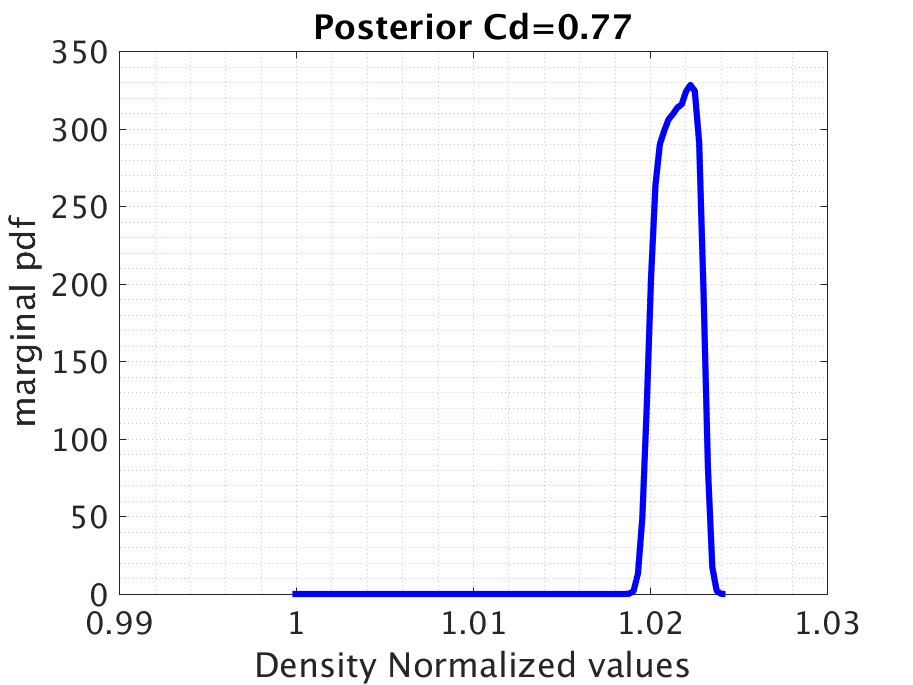
\includegraphics[width=1.1\textwidth,keepaspectratio]{images/inverse_problem/infer_radius/0_77/densityraw_PDF.png}
    \caption{\centering Cd=0.77}
  \end{subfigure}
 %%\hspace{1.5cm}%
 \begin{subfigure}{0.4\textwidth}
    \centering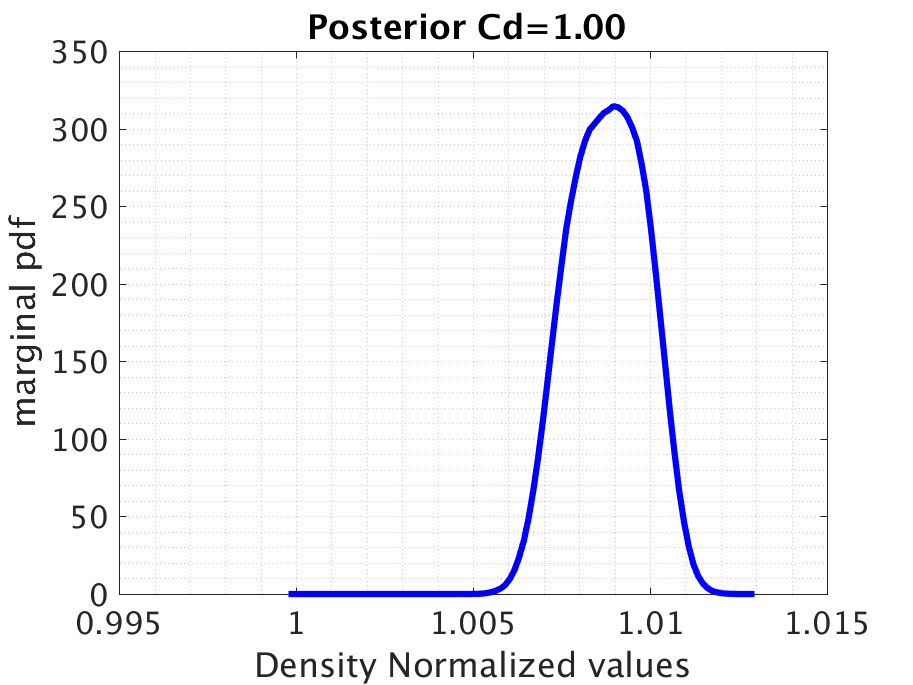
\includegraphics[width=1.1\textwidth,keepaspectratio]{images/inverse_problem/infer_radius/drag_01/densityraw_PDF.png}
    \caption{\centering Cd=1.00}
  \end{subfigure}
  \begin{subfigure}{0.4\textwidth}
    \centering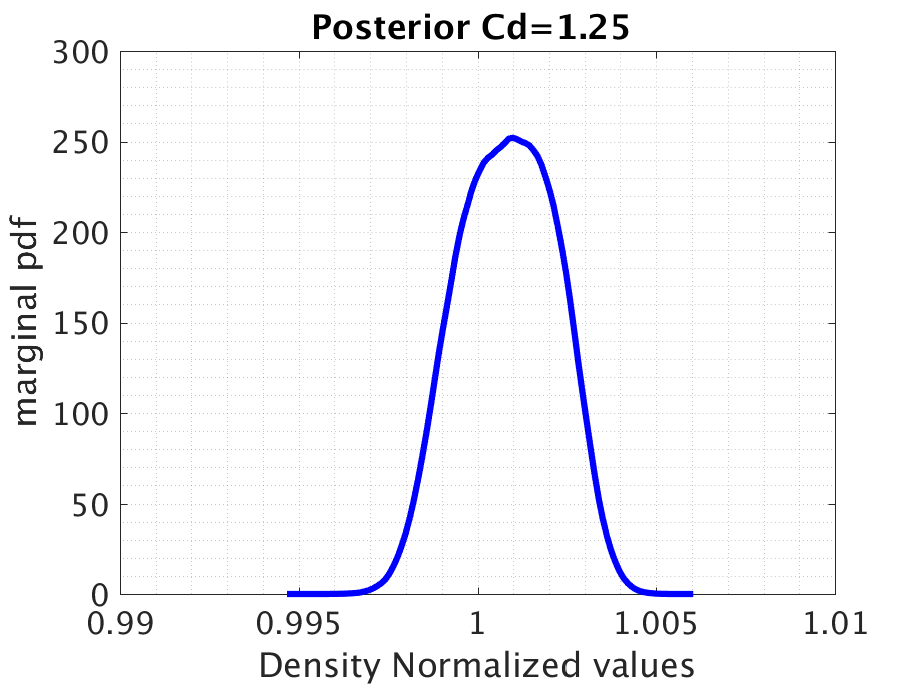
\includegraphics[width=1.1\textwidth,keepaspectratio]{images/inverse_problem/infer_radius/drag_125/range_short/densityraw_PDF.png}
    \caption{\centering Cd=1.25}
  \end{subfigure}
  \begin{subfigure}{0.4\textwidth}
    \centering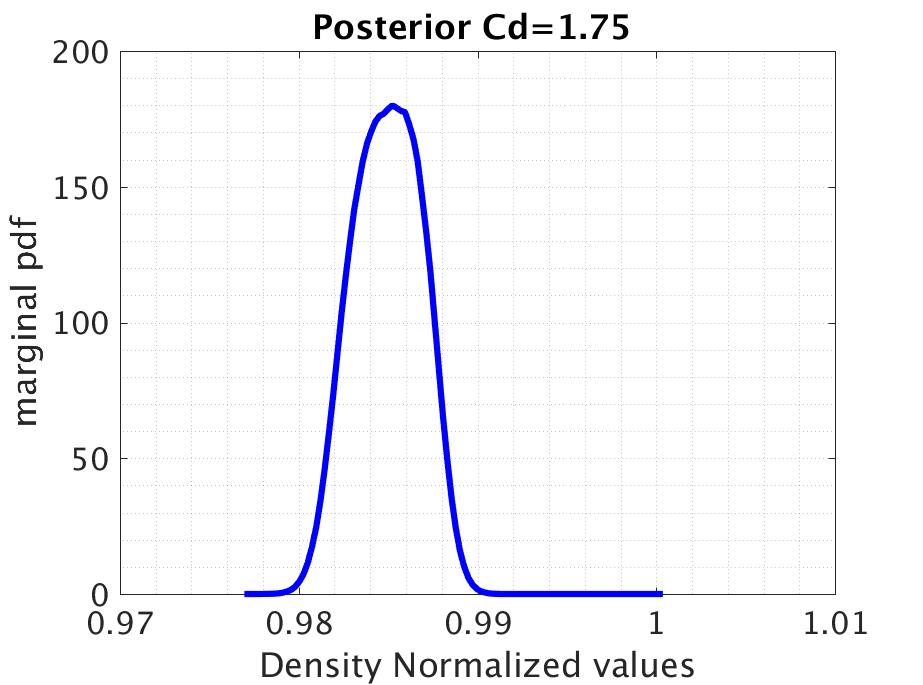
\includegraphics[width=1.1\textwidth,keepaspectratio]{images/inverse_problem/infer_radius/drag_175/densityraw_PDF.png}
    \caption{\centering Cd=1.75}
  \end{subfigure}

\caption{Droplet density PDF for different CD's .}
\label{fig:first_compilation} 
 \end{center}
\end{figure}



In the previous section we have demonstrate that one possible value of the drag coefficient for our experiment was approximately $0.77$ but analyzing the figure \ref{fig:first_compilation} we can see that this value gives a posterior distribution quite  separated from the nominal value ( which is represented as the value of 1). For the figure (b) we have the same problem but in this case we can note that we are getting close to the right value which may be $Cd=1.25$ as the posterior distribution is practically centered at 1. Finally it can be seen in the figure (c) that if we give high values to the drag coefficient the density tends to decrease which may lead us to conclude that the density is inversely  proportional to the drag coefficient which is not true so we need to take care of this kind of conclusions an be aware at all moments the problem we are analyzing. In the same way is important analyze the density distribution in order to avoid values higher than the water density as in this case the problem has no sense.
 \par \noindent
 At this point we 
 

we can use the histograms to see in a best visual way the change in distribution
Then regarding your last comment π(ρ∈[0.6,0.8]|data)π(ρ∈[0.6,0.8]|data) represents the belief ρρ is in [0.6,0.8][0.6,0.8] after having observed the data. Conversely the highest posterior density (HPD) interval (which will be something close to [0.6,0.8] in your case), gives you the smallest interval covering a given subset (typical 95%) of the belief and can be interpreted as a reasonable range for the actual value of ρρ (when the posterior in unimodal).

There is another interesting point regarding the different output files we can get  from QUESO. Is the case of the filtered chains. The interested in the filtered chain is due to the fact that for many problems is important to retain the information of the posterior distribution. However storing all the information can  very expensive in terms of memory and processing. Is when the filtered chain makes sense because this chain is not  essential in this problem, but can be very important for sequential processing where new data is processed upon arrival in a short period of time and is also needed save as much memory as possible.
 \par \noindent
In thh figure \ref{fig:raw_filtered} it can be seen the PDf and the histogram for the whole chain (raw chain) and the filtered one. As the figures show, the confidence interval is very similar for two chains considering that the number of samples are 2 million for the raw chain and only 1000 samples for the filtered chain.


\begin{figure}[H]
\captionsetup[subfigure]{justification=centering}
\begin{center}
  \begin{subfigure}{0.4\textwidth}
    \centering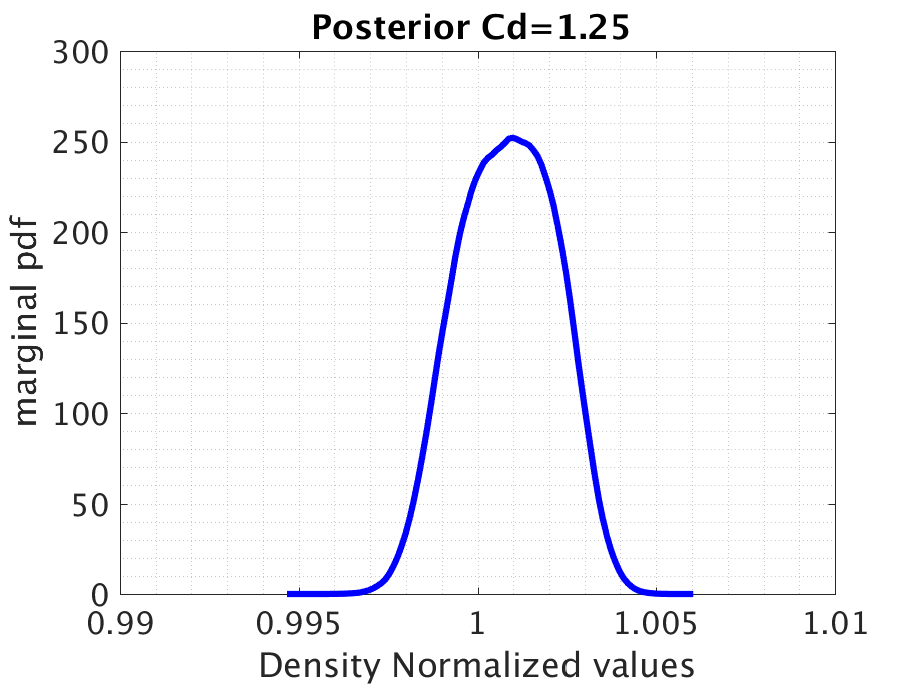
\includegraphics[width=1.1\textwidth,keepaspectratio]{images/inverse_problem/infer_radius/drag_125/range_short/densityraw_PDF.png}
    \caption{\centering PDF raw chain}
  \end{subfigure}
 %%\hspace{1.5cm}%
 \begin{subfigure}{0.4\textwidth}
    \centering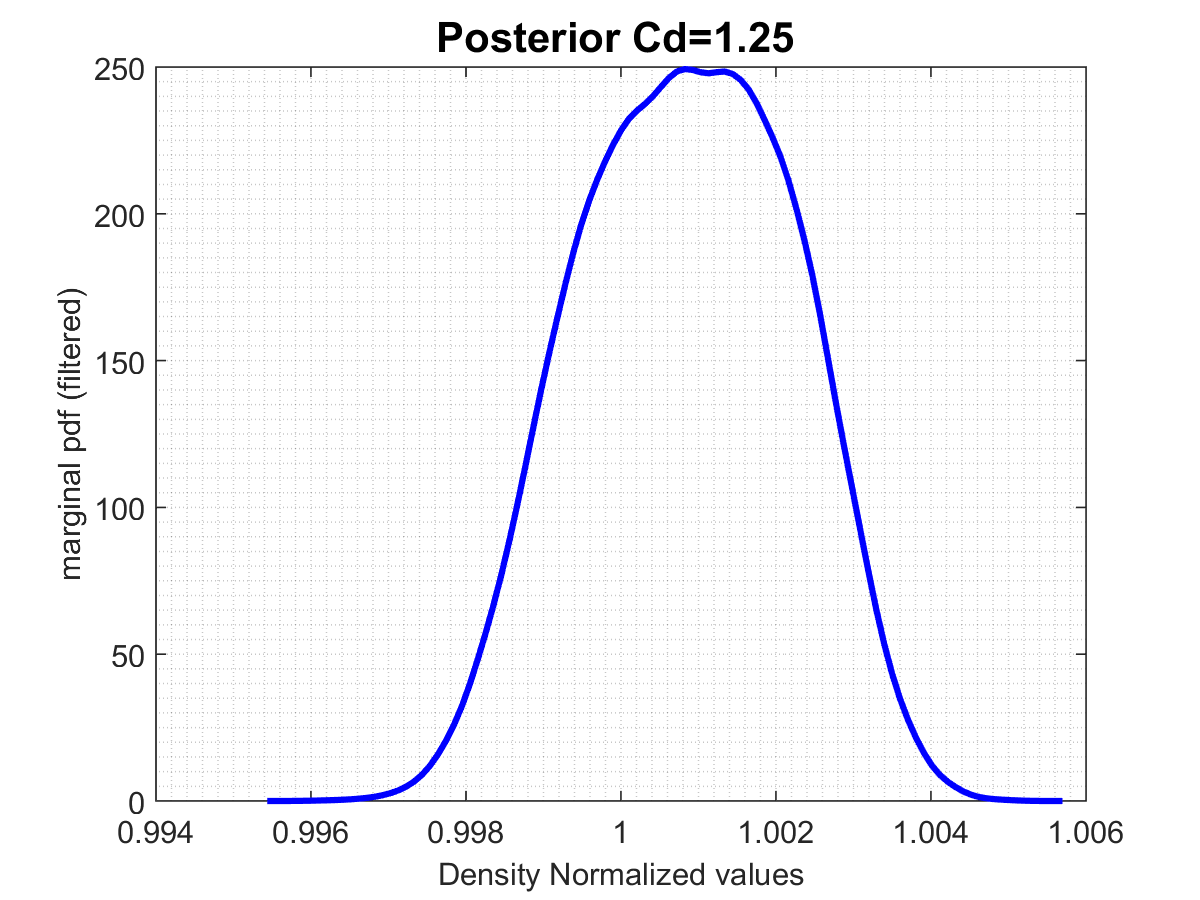
\includegraphics[width=1.1\textwidth,keepaspectratio]{images/inverse_problem/infer_radius/drag_125/range_short/densityfiltered_PDF.png}
    \caption{\centering PDF filtered chain}
  \end{subfigure}
  \begin{subfigure}{0.4\textwidth}
    \centering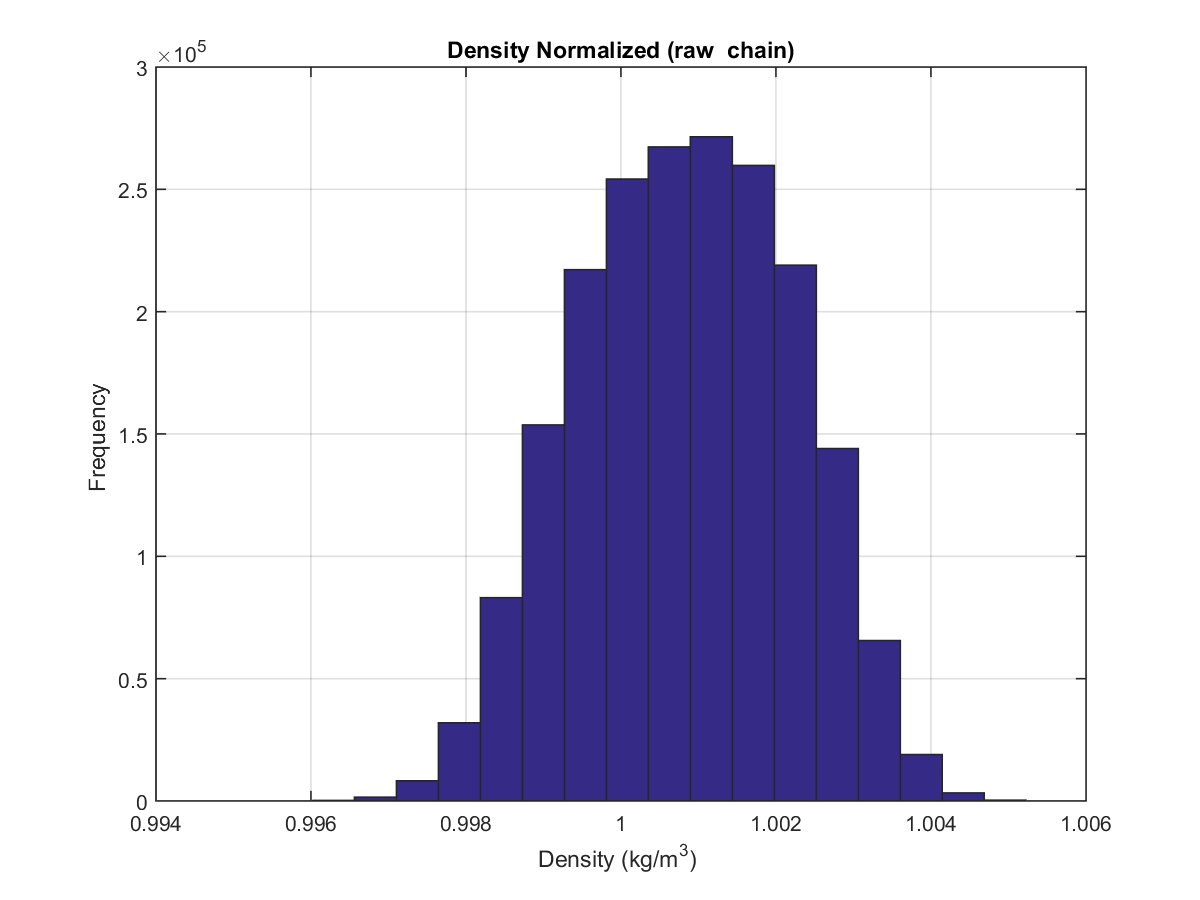
\includegraphics[width=1.1\textwidth,keepaspectratio]{images/inverse_problem/infer_radius/drag_125/range_short/density_histogram_raw.png}
    \caption{\centering Histogram raw chain}
  \end{subfigure}
  \begin{subfigure}{0.4\textwidth}
    \centering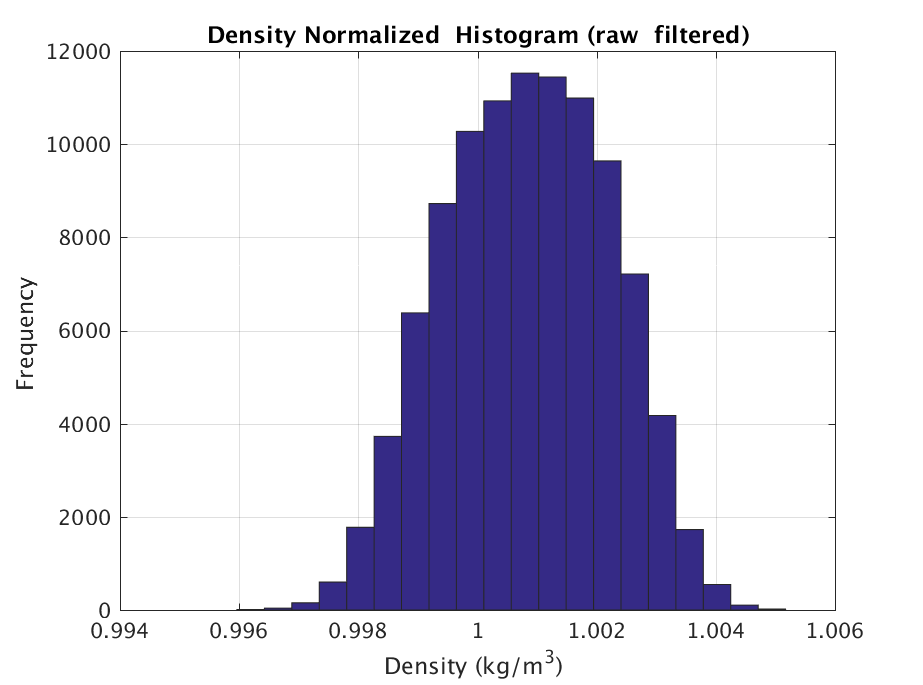
\includegraphics[width=1.1\textwidth,keepaspectratio]{images/inverse_problem/infer_radius/drag_125/range_short/density_histogram_filtered.png}
    \caption{\centering Histogram filtered chain}
  \end{subfigure}

\caption{PDF and Histogram for the raw and filtered chain}
\label{fig:raw_filtered} 
 \end{center}
\end{figure}


Additionally,  is also  interesting analyzing the effect that the uncertainty has over the density distribution. It has been explained that in the input file the prior information is set. So, for the case of the radius parameter an interval has been chosen based on the experiment. But what happens if the prior interval of the radius  gets longer.  In this case the uncertainty of knowing the radius is higher and this change affects to the posterior distribution (figure \ref{fig:results_interval}) .



\begin{figure}[H]
\captionsetup[subfigure]{justification=centering}
\begin{center}
  \begin{subfigure}{0.4\textwidth}
    \centering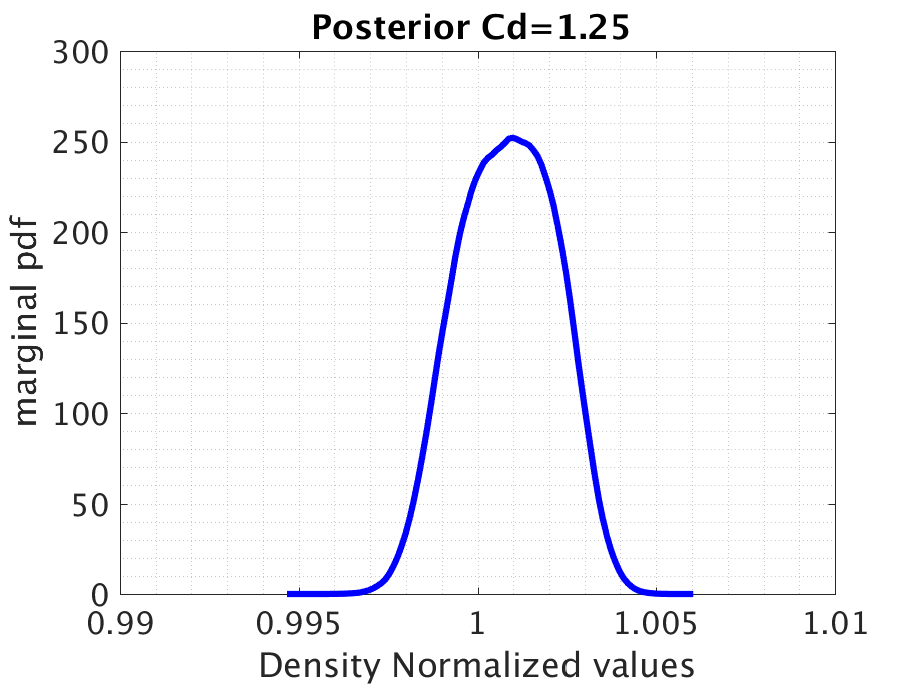
\includegraphics[width=1.1\textwidth,keepaspectratio]{images/inverse_problem/infer_radius/drag_125/range_short/densityraw_PDF.png}
    \caption{\centering PDF  $R_d$ in [0.95-1.05]}
  \end{subfigure}
 %%\hspace{1.5cm}%
 \begin{subfigure}{0.4\textwidth}
    \centering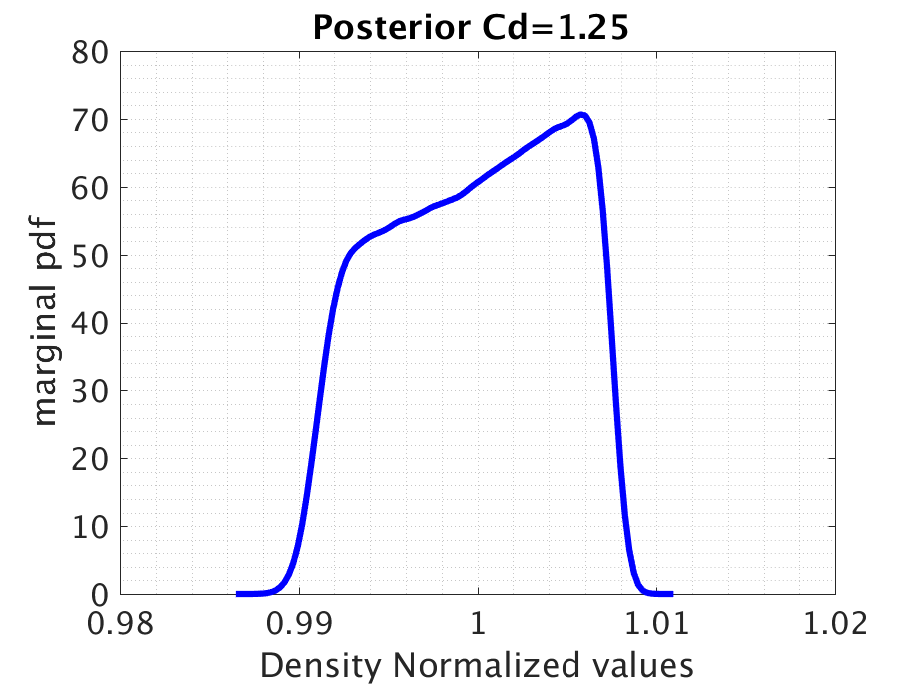
\includegraphics[width=1.1\textwidth,keepaspectratio]{images/inverse_problem/infer_radius/drag_125/range_long/densityraw_PDF.png}
    \caption{\centering PDF  $R_d$ in [0.8-1.2]}
  \end{subfigure}
  \begin{subfigure}{0.4\textwidth}
    \centering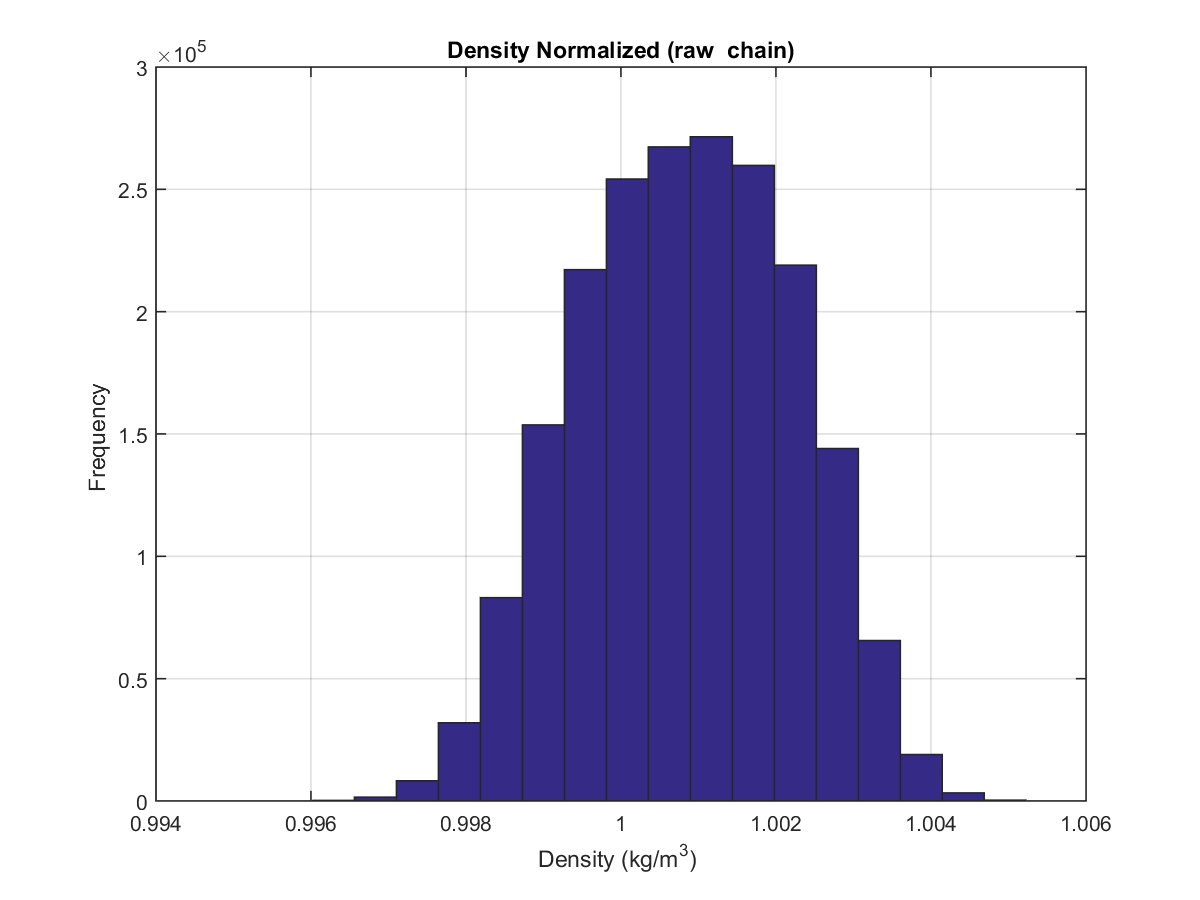
\includegraphics[width=1.1\textwidth,keepaspectratio]{images/inverse_problem/infer_radius/drag_125/range_short/density_histogram_raw.png}
    \caption{\centering Histogram$R_d$ in [0.95-1.05]}
  \end{subfigure}
  \begin{subfigure}{0.4\textwidth}
    \centering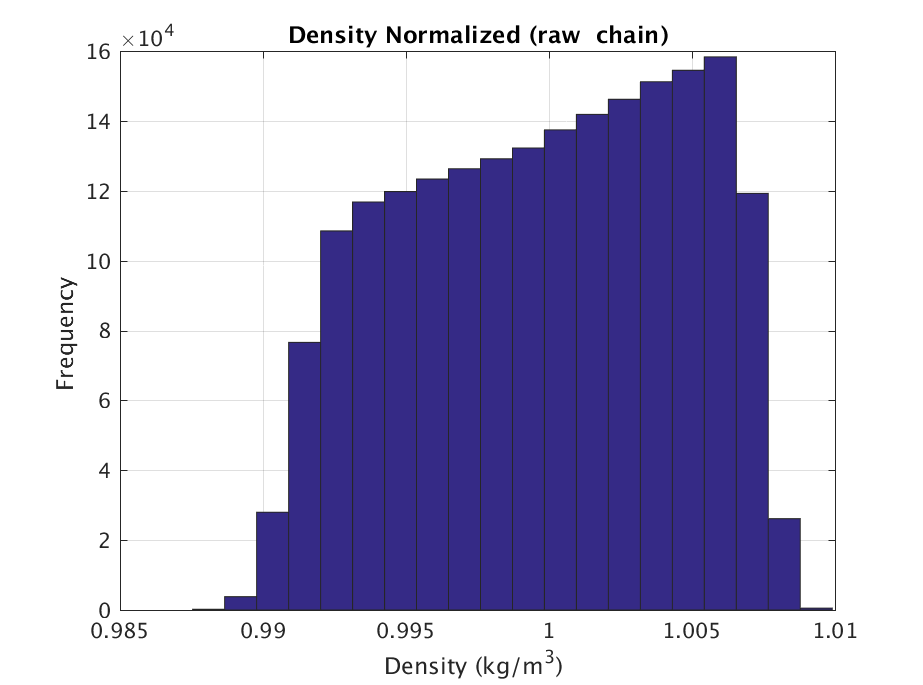
\includegraphics[width=1.1\textwidth,keepaspectratio]{images/inverse_problem/infer_radius/drag_125/range_long/density_histogram_raw.png}
    \caption{\centering Histogram $R_d$ in [0.8-1.2]}
  \end{subfigure}

\caption{PDF and Histogram varying the prior radius interval.}
\label{fig:results_interval} 
 \end{center}
\end{figure}

It can be noted that the fact of increasing the uncertainty in the radius interval makes a change in the posterior distributions. So, the effect of the uncertainty leads to an increase of the confidence interval for droplet density posterior although the distribution is practically centered to the real value ( the mean is over 1).

Finally, in the figure \ref{fig:radius_interval} the results for the radius posterior distribution are plotted.  Basically,  for both cases there is no variation respect to the prior interval, which means that there is no extra information got from the data space (in this case we just get the information of the radius for each sample). For getting results more accurate we would need more information in the data space.
\begin{figure}[H]
\captionsetup[subfigure]{justification=centering}
\begin{center}
  \begin{subfigure}{0.4\textwidth}
    \centering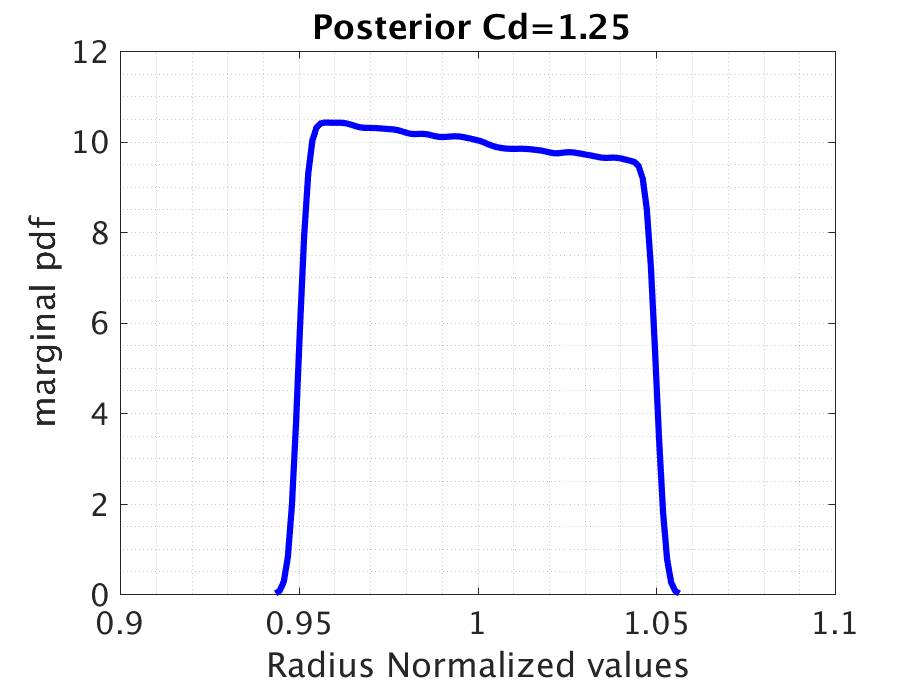
\includegraphics[width=1.1\textwidth,keepaspectratio]{images/inverse_problem/infer_radius/drag_125/range_short/radiusraw_PDF.png}
    \caption{\centering Radius PDF  $R_d$ in [0.95-1.05]}
  \end{subfigure}
 %%\hspace{1.5cm}%
 \begin{subfigure}{0.4\textwidth}
    \centering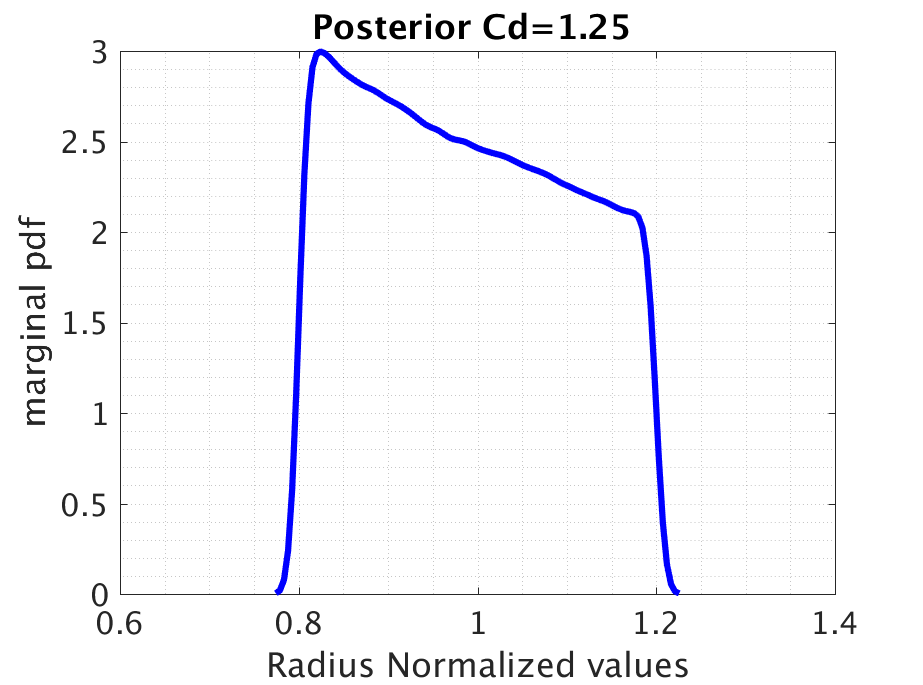
\includegraphics[width=1.1\textwidth,keepaspectratio]{images/inverse_problem/infer_radius/drag_125/range_long/radiusraw_PDF.png}
    \caption{\centering Radius PDF  $R_d$ in [0.8-1.2]}
  \end{subfigure}


\caption{PDF and Histogram varying the prior radius interval.}
\label{fig:radius_interval} 
 \end{center}
\end{figure}

These rules of thumb follow directly from the nature of the Bayesian analysis procedure:

If the prior is uninformative, the posterior is very much determined by the data (the posterior is data-driven)
If the prior is informative, the posterior is a mixture of the prior and the data
The more informative the prior, the more data you need to "change" your beliefs, so to speak because the posterior is very much driven by the prior information
If you have a lot of data, the data will dominate the posterior distribution (they will overwhelm the prior).




















%\bibliographystyle{plain}
%\bibliography{bibliography/sample2}{}


\end{document}